\documentclass[twocolumn]{article}
\usepackage[utf8]{inputenc}
\usepackage[linesnumbered,ruled,vlined]{algorithm2e} 

\title{Lab Report}
\author{Your name here}
\date{\today}   % You can use \date{\today}

\usepackage{biblatex}
\addbibresource{references.bib}
\usepackage{graphicx}
\usepackage{hyperref}
\usepackage{color}

\begin{document}

\maketitle

\section{Introduction}

{\color{red} CAREFUL! This report has a limit of 4 pages plus the references. This means $\leq 4$ everything except the bibliography }\\

You can use Overleaf to edit the report. Make a copy of this template, as shown in Figure \ref{fig:copyproject} and edit it. The algorithm \ref{main_algorithm} tells you how to create a copy of this example (and how to write a simple algorithm with Latex). You can also check the online documentation \cite{OverleafHelp}.

The introduction should consist of:
\begin{itemize}
    \item A list of the problems that you are solving for the 10 points (IMPORTANT: choose exercises for only 10 points and no more. All exercises that exceeds the first 10 points will not count for your final grade).
    \item Brief explanation of the problems you are addressing (you can include fundamentals, notation. references to materials you used among others). You should try to unify the explanations, if possible, specially of the problems from the same lab or topic.
    \item A recommended size for the introduction would be about half a page and \textbf{the full report should be five pages or less (excluding references)}.
\end{itemize}

To cite a bibliographic source, you must include the corresponding entry in the .bib file and \emph{cite that source within the text} \cite{OverleafBibTexHelp} (using the \texttt{cite} command)


To insert an image you just have to follow the example in Fig. \ref{fig:CNN}. The image is not original made by us, so it needs a citation to acknowledge its source. Since it has been taken from Wikicommons, the attribution has been generated with "Attribution Generator"\cite{AttributionGenerator}.
  If the figure is yours, indeed there is no need for attribution. \\


\begin{figure}[!htb]
\centering
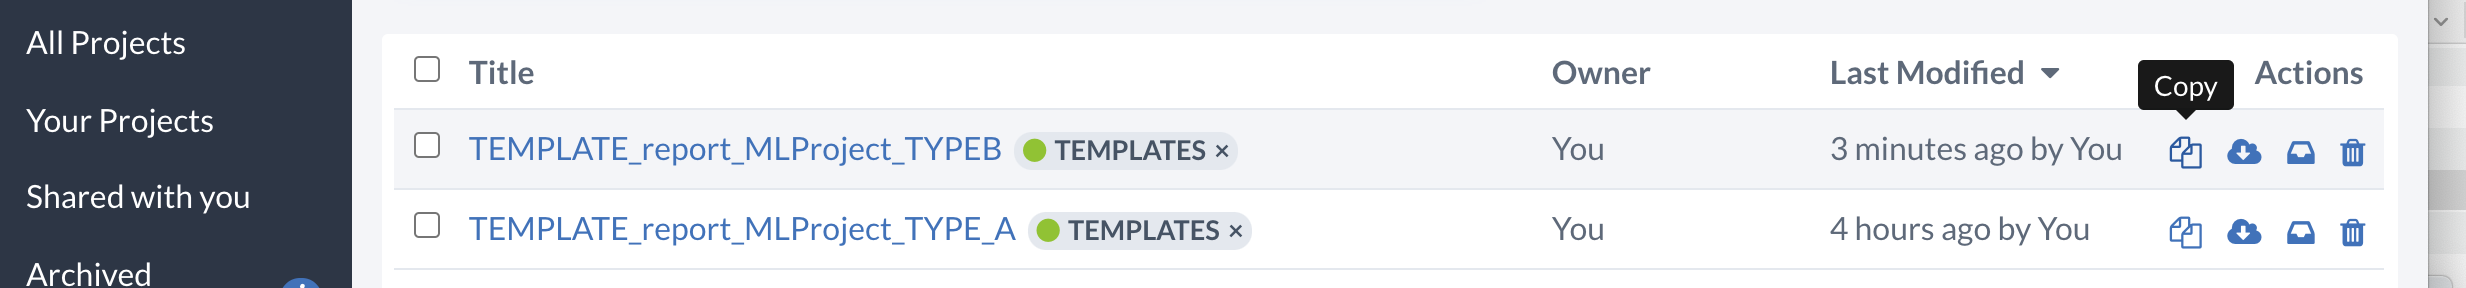
\includegraphics[width=0.95\columnwidth]{images/copyproject.png}
\caption{Copy project overleaf}
\label{fig:copyproject}
\end{figure}
  
\section{Lab or Exercise 1}

You can break the report in exercises or, even better, in labs or related exercises. Briefly introduce the concepts of the exercise. Important: \textbf{do not} repeat the exercise statement. We already know it, we wrote it.


\subsection{Theoretical background}

\paragraph{Problem formulation (one paragraph).} 
Description of the mathematical formulation of the problem, explaining the mathematical notation. Provide a connection with the theory from the lectures. If needed, formulate at least the most important equation that represents the classification / segmentation / regression (etc ...) problem that you are solving. For every equation you need to make sure that all variables used are defined are explained in the text around the equation:

\paragraph{Equations:} This is a toy example description of equation (\ref{eq:linear}):

\textit{Our classifier score function $f$ is computed as follows:}
\begin{equation}
s_i = f(x_i) = W_1 x_i + b, \label{eq:linear}
\end{equation}
\noindent where $W_1$ and $b$ are the weights and bias of the function respectively, $x_i$ is the $i^{th}$ input sample and $s_i$ is the score computed for that sample.


\paragraph{Algorithm:} Instead of equations, you might also provide a high-level description of the algorithm (See Algorithm \ref{main_algorithm}) or model used in the exercise or lab (as summarized in the diagram from Fig.~\ref{fig:CNN}). 

\subsection{Implementation and validation}
You should highlight why you applied a particular solution to the problem. Justify the code or approach selected and the motivation for each component. Connect it with the problem formulation that you have defined above or with related topics seen in class. You should avoid describing the code (it should be self-documented) or paraphrasing the slides.

\begin{algorithm}[!tb]
 \KwData{A sample doc in Overleaf}
 \KwResult{Your own copy to fill up and prepare your report}
 \If{you do not have a Overleaf account}{
   Create account\;
 }
 
 \uIf{you open this template from your overleaf account}{
   Make directly a copy as shown in Fig.~\ref{fig:copyproject}\;
 }
 \uElseIf{you download this project source with Menu-Download-source}{
    Create New Project with the option select Upload Project\;
    Load modelOverleafPractica.zip\;
 }
 \Else{
    Ask for help :-) \;
 }
 
 \While{not finished}{
   write, add figures, ...\;
   recompile\;
 }
 \caption{How to get your Overleaf report ready}
 \label{main_algorithm}
\end{algorithm}



\begin{figure}[!htb]
\centering
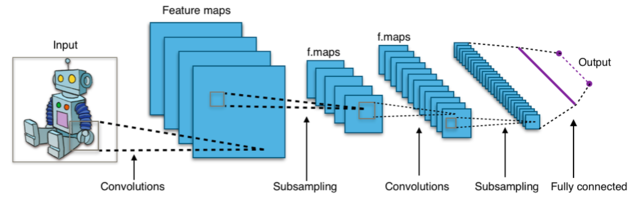
\includegraphics[width=\columnwidth]{images/640px-Typical_cnn.png}
\caption{Typical architecture of a CNN. {\footnotesize (Source: By Aphex34, CC BY-SA 4.0, \url{https://commons.wikimedia.org/w/index.php?curid=45679374})}}
\label{fig:CNN}
\end{figure}


\paragraph{Experimental Validation:} If the exercise included an experimental validation, you should report your results here, including a description of any \textbf{dataset} that you have used and was not provided with the lab and the \textbf{metrics} that you have used for evaluation. You can condense the results in a table for better visualisation (see Table~\ref{tab:results}).

\begin{table}
\begin{center}
\begin{tabular}{|c||c|c|}
\hline
Method & Accuracy [\%] & Cost [s] \\ 
\hline
\hline
A cool method & $78.7$ & $376.7$ \\ 
\hline
The coolest method & $89.4$ & $23.2$ \\ 
\hline
\end{tabular}
\end{center}
\caption{My results. Notice how the coolest method outperforms the cool one in accuracy and cost.}
\label{tab:results}
\end{table}

\section{Conclusion}
Discuss the main conclusions you can draw from the labs that you have performed. Similarly to the introduction, you should try to unify the conclusions of related exercises or labs.


\printbibliography
\end{document}